\documentclass[hide notes,intlimits]{beamer}


\mode<presentation>
{
  \usetheme[footline]{UAFshade}
  \setbeamercovered{transparent}
}

% load packages
\usepackage{media9}
\usepackage{movie15}
\usepackage[english]{babel}
\usepackage[latin1]{inputenc}
\usepackage[T1]{fontenc}
\usepackage{lmodern}
\usepackage[multidot]{grffile}

\usepackage{tikz}
\usetikzlibrary{shapes,arrows,shadows, calc}

\definecolor{dark red}{HTML}{E41A1C}
\definecolor{dark green}{HTML}{4DAF4A}
\definecolor{dark violet}{HTML}{984EA3}
\definecolor{dark blue}{HTML}{084594}
\definecolor{dark orange}{HTML}{FF7F00}
\definecolor{light blue}{HTML}{377EB8}
\definecolor{light red}{HTML}{FB9A99}
\definecolor{light violet}{HTML}{CAB2D6}

\definecolor{uaf red}{HTML}{E41A1C}
\definecolor{uaf blue}{HTML}{377EB8}
\definecolor{uaf green}{HTML}{4DAF4A}
\definecolor{uaf violet}{HTML}{984EA3}
\definecolor{uaf orange}{HTML}{FF7F00}
\setbeamercolor{boxed}{fg=black,bg=uaf yellow}

\graphicspath{{figures/}}

\setbeamerfont{caption}{size=\scriptsize}

% code adapted from http://tex.stackexchange.com/a/11483/3954

% some parameters for customization
\def\shadowshift{3pt,-3pt}
\def\shadowradius{6pt}

\colorlet{innercolor}{black!60}
\colorlet{outercolor}{gray!05}

% this draws a shadow under a rectangle node
\newcommand\drawshadow[1]{
    \begin{pgfonlayer}{shadow}
        \shade[outercolor,inner color=innercolor,outer color=outercolor] ($(#1.south west)+(\shadowshift)+(\shadowradius/2,\shadowradius/2)$) circle (\shadowradius);
        \shade[outercolor,inner color=innercolor,outer color=outercolor] ($(#1.north west)+(\shadowshift)+(\shadowradius/2,-\shadowradius/2)$) circle (\shadowradius);
        \shade[outercolor,inner color=innercolor,outer color=outercolor] ($(#1.south east)+(\shadowshift)+(-\shadowradius/2,\shadowradius/2)$) circle (\shadowradius);
        \shade[outercolor,inner color=innercolor,outer color=outercolor] ($(#1.north east)+(\shadowshift)+(-\shadowradius/2,-\shadowradius/2)$) circle (\shadowradius);
        \shade[top color=innercolor,bottom color=outercolor] ($(#1.south west)+(\shadowshift)+(\shadowradius/2,-\shadowradius/2)$) rectangle ($(#1.south east)+(\shadowshift)+(-\shadowradius/2,\shadowradius/2)$);
        \shade[left color=innercolor,right color=outercolor] ($(#1.south east)+(\shadowshift)+(-\shadowradius/2,\shadowradius/2)$) rectangle ($(#1.north east)+(\shadowshift)+(\shadowradius/2,-\shadowradius/2)$);
        \shade[bottom color=innercolor,top color=outercolor] ($(#1.north west)+(\shadowshift)+(\shadowradius/2,-\shadowradius/2)$) rectangle ($(#1.north east)+(\shadowshift)+(-\shadowradius/2,\shadowradius/2)$);
        \shade[outercolor,right color=innercolor,left color=outercolor] ($(#1.south west)+(\shadowshift)+(-\shadowradius/2,\shadowradius/2)$) rectangle ($(#1.north west)+(\shadowshift)+(\shadowradius/2,-\shadowradius/2)$);
        \filldraw ($(#1.south west)+(\shadowshift)+(\shadowradius/2,\shadowradius/2)$) rectangle ($(#1.north east)+(\shadowshift)-(\shadowradius/2,\shadowradius/2)$);
    \end{pgfonlayer}
}

% create a shadow layer, so that we don't need to worry about overdrawing other things
\pgfdeclarelayer{shadow} 
\pgfsetlayers{shadow,main}

\newsavebox\mybox
\newlength\mylen

\newcommand\shadowimage[2][]{%
\setbox0=\hbox{\includegraphics[#1]{#2}}
\setlength\mylen{\wd0}
\ifnum\mylen<\ht0
\setlength\mylen{\ht0}
\fi
\divide \mylen by 120
\def\shadowshift{\mylen,-\mylen}
\def\shadowradius{\the\dimexpr\mylen+\mylen+\mylen\relax}
\begin{tikzpicture}
\node[anchor=south west,inner sep=0] (image) at (0,0) {\includegraphics[#1]{#2}};
\drawshadow{image}
\end{tikzpicture}}

\newcommand\shadowimagec[3][]{%
\setbox0=\hbox{\includegraphics<#1>[#2]{#3}}
\setlength\mylen{\wd0}
\ifnum\mylen<\ht0
\setlength\mylen{\ht0}
\fi
\divide \mylen by 120
\def\shadowshift{\mylen,-\mylen}
\def\shadowradius{\the\dimexpr\mylen+\mylen+\mylen\relax}
\begin{tikzpicture}
\node[anchor=south west,inner sep=0] (image) at (0,0) {\includegraphics<#1>[#2]{#3}};
\drawshadow{image}
\end{tikzpicture}}


\newenvironment{transbox}[1][]{%
\begin{tikzpicture}
\node[drop shadow,rounded corners,text width=\textwidth,fill=white, fill opacity=#1,text opacity=1] \bgroup
}{
\egroup;\end{tikzpicture}} 

\newenvironment{transbox-tight}{%
\begin{tikzpicture}
\node[drop shadow,rounded corners,fill=uaf yellow, fill opacity=0.75,text opacity=1] \bgroup
}{
\egroup;\end{tikzpicture}} 


% title page
\title[] % (optional, use only with long paper titles)
{Complex Greenland Outlet Glacier Flow Captured}


\author[Aschwanden, Fahnestock, Truffer] % (optional, use only with lots of authors)
{Andy Aschwanden, Mark Fahnestock \& Martin Truffer}
% - Give the names in the same order as the appear in the paper.
% - Use the \inst{?} command only if the authors have different
%   affiliation.

\institute[Geophysical Institute] % (optional, but mostly needed)
{}
% - Use the \inst command only if there are several affiliations.
% - Keep it simple, no one is interested in your street address.

\titlegraphic{\vskip-0.5cm\includegraphics[width=\textwidth]{gris-nw-speed-exp-600m}}

\date{}

\begin{document}

% define what is shown at the beginning of each section
\AtBeginSection[]
{
  \begin{frame}<handout:0>
    \frametitle{Outline}
   \tableofcontents[currentsection,subsectionstyle=hide/hide/hide]
  \end{frame}
}

% define what is shown at the beginning of each subsection
\AtBeginSubsection[]
{
 \begin{frame}<beamer>
  \frametitle{Outline}
   \tableofcontents[currentsection,currentsubsection]
 \end{frame}
}

\setbeamertemplate{background canvas}
  {
     \tikz{\node[inner sep=0pt,opacity=1.0] {\includegraphics[width=\paperwidth]{uaf_beamer_shade_bg}};}
} 


% insert titlepage
\begin{frame}
  \titlepage
  \note[item]{talk is somewhat unfinished and I'm likely to get lost towards the end\ldots}
  \note[item]{this work has emerged from a close collaboration with Mark Fahnestock and Martin Truffer}
  \note[item]{I merely pushed some buttons}
  \note[item]{my talk will illustrate one of the most basic principles of glaciology: ice thickness matters}
\end{frame}


\setbeamertemplate{background canvas}
{
%
} 

% \begin{frame}[plain]
%   \includemedia[width=\textwidth,
%   height=\textheight,
%   addresource=grace_greenland_2004_2013_1080p.mp4,
%   flashvars={source=grace_greenland_2004_2013_1080p.mp4}
% ]{foo}{grace_greenland_2004_2013_1080p.mp4}
% \end{frame}

% \begin{frame}[plain]
%   \includemedia[width=\paperwidth,
%   height=\paperheight,
%   addresource=random.flv,
%   flashvars={source=random.flv,
%     &autoPlay=true},
% ]{foo}{random.flv}
% \end{frame}

\begin{frame}[plain]
  \begin{figure}[ht]
    \includemovie[text={\small(Loading Video...)}]{\paperwidth}{\paperheight}{grace_greenland_2004_2013_1080p.mp4}
  \end{figure}\end{frame}

\begin{frame}{The beginning of Greenland ice flow modeling}
  \begin{columns}
    \column[c]{4.25cm}
    \begin{figure}
      \includegraphics<1>[height=.65\textheight]{greve_1997_mass_flux}
      \small 
      \caption{Simulated ass flux (SICOPOLIS) from Greve (1997)}
    \end{figure}
    \column[c]{6.75cm}
    \begin{itemize}
      \item started in the mid-1990's
      \item pioneered by R. Greve, P. Huybrechts, C. Ritz and others
      \item based on the Shallow Ice Approximation
      \item horizontal grid size: 20--40\,km
    \end{itemize}
  \end{columns}
\end{frame}


\begin{frame}{Observed flow: pre-SAR era}
  \begin{columns}
    \column[c]{2.75cm}
    \begin{figure}
      \shadowimage[width=\textwidth]{stake-measurement-gulkana}
      \caption{credit: L. Sass, USGS}
    \end{figure}
    \column[c]{8.5cm}
    \begin{itemize}
    \item spatial and temporal coverage was very limited
    \item mostly point measurements, e.g.
    \begin{itemize}
    \item Jakobshavn Isbr{\ae} (e.g. Echelmeyer, 1990)
    \item EGIG, PARCA 2000\,m velocity line
    \end{itemize}
  \item it was already known that Jakobshavn Isbr{\ae} is flowing fast
  \end{itemize}
\end{columns}
\end{frame}


\begin{frame}{Observed flow: SAR era}
  \begin{columns}
    \column[c]{2.5cm}
    \begin{figure}
      \shadowimage[width=\textwidth]{sar-sentinel}
    \end{figure}
    \column[c]{8.5cm}
    \begin{itemize}
    \item pioneered by I. Joughin, E. Rignot, M. Fahnestock
    \item ERS1/2 and RADARSAT
    \item reveals large spatial and temporal flow variability
    \end{itemize}
  \end{columns}
  \begin{figure}
    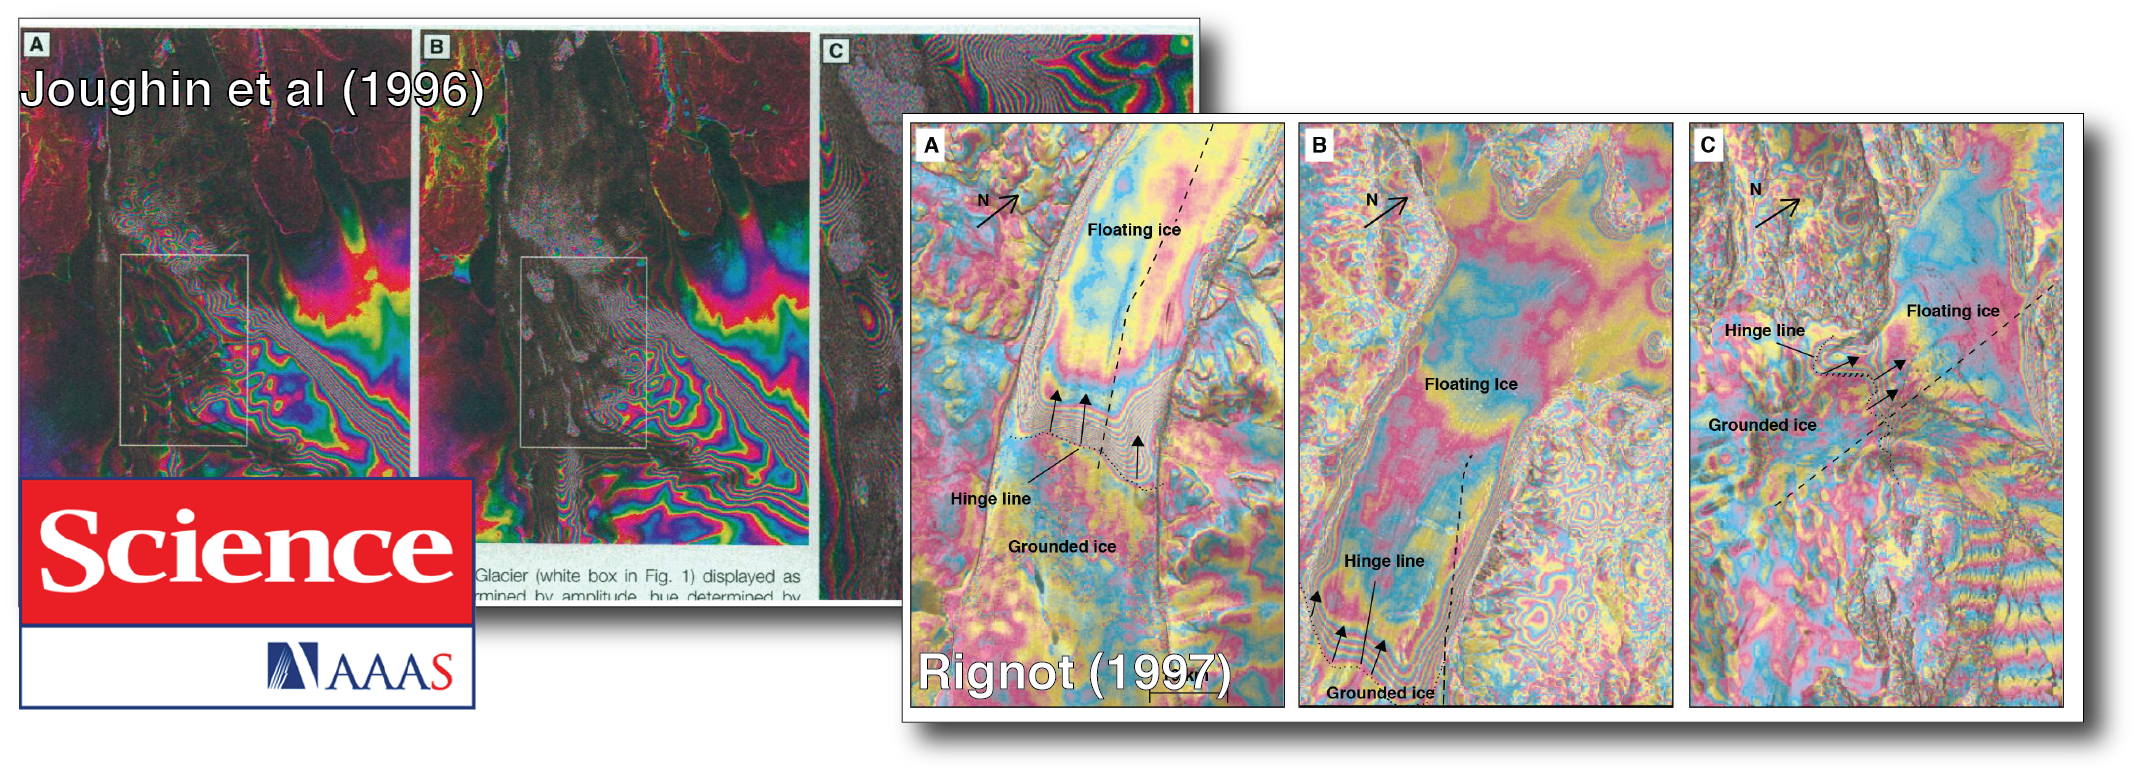
\includegraphics[width=\textwidth]{gris-early-sar}
  \end{figure}
\end{frame}


\begin{frame}{Observed spatial flow variability}
  nearly-perfect spatial coverage but non-negligible uncertainties in slow-flowing areas
  \begin{figure}
    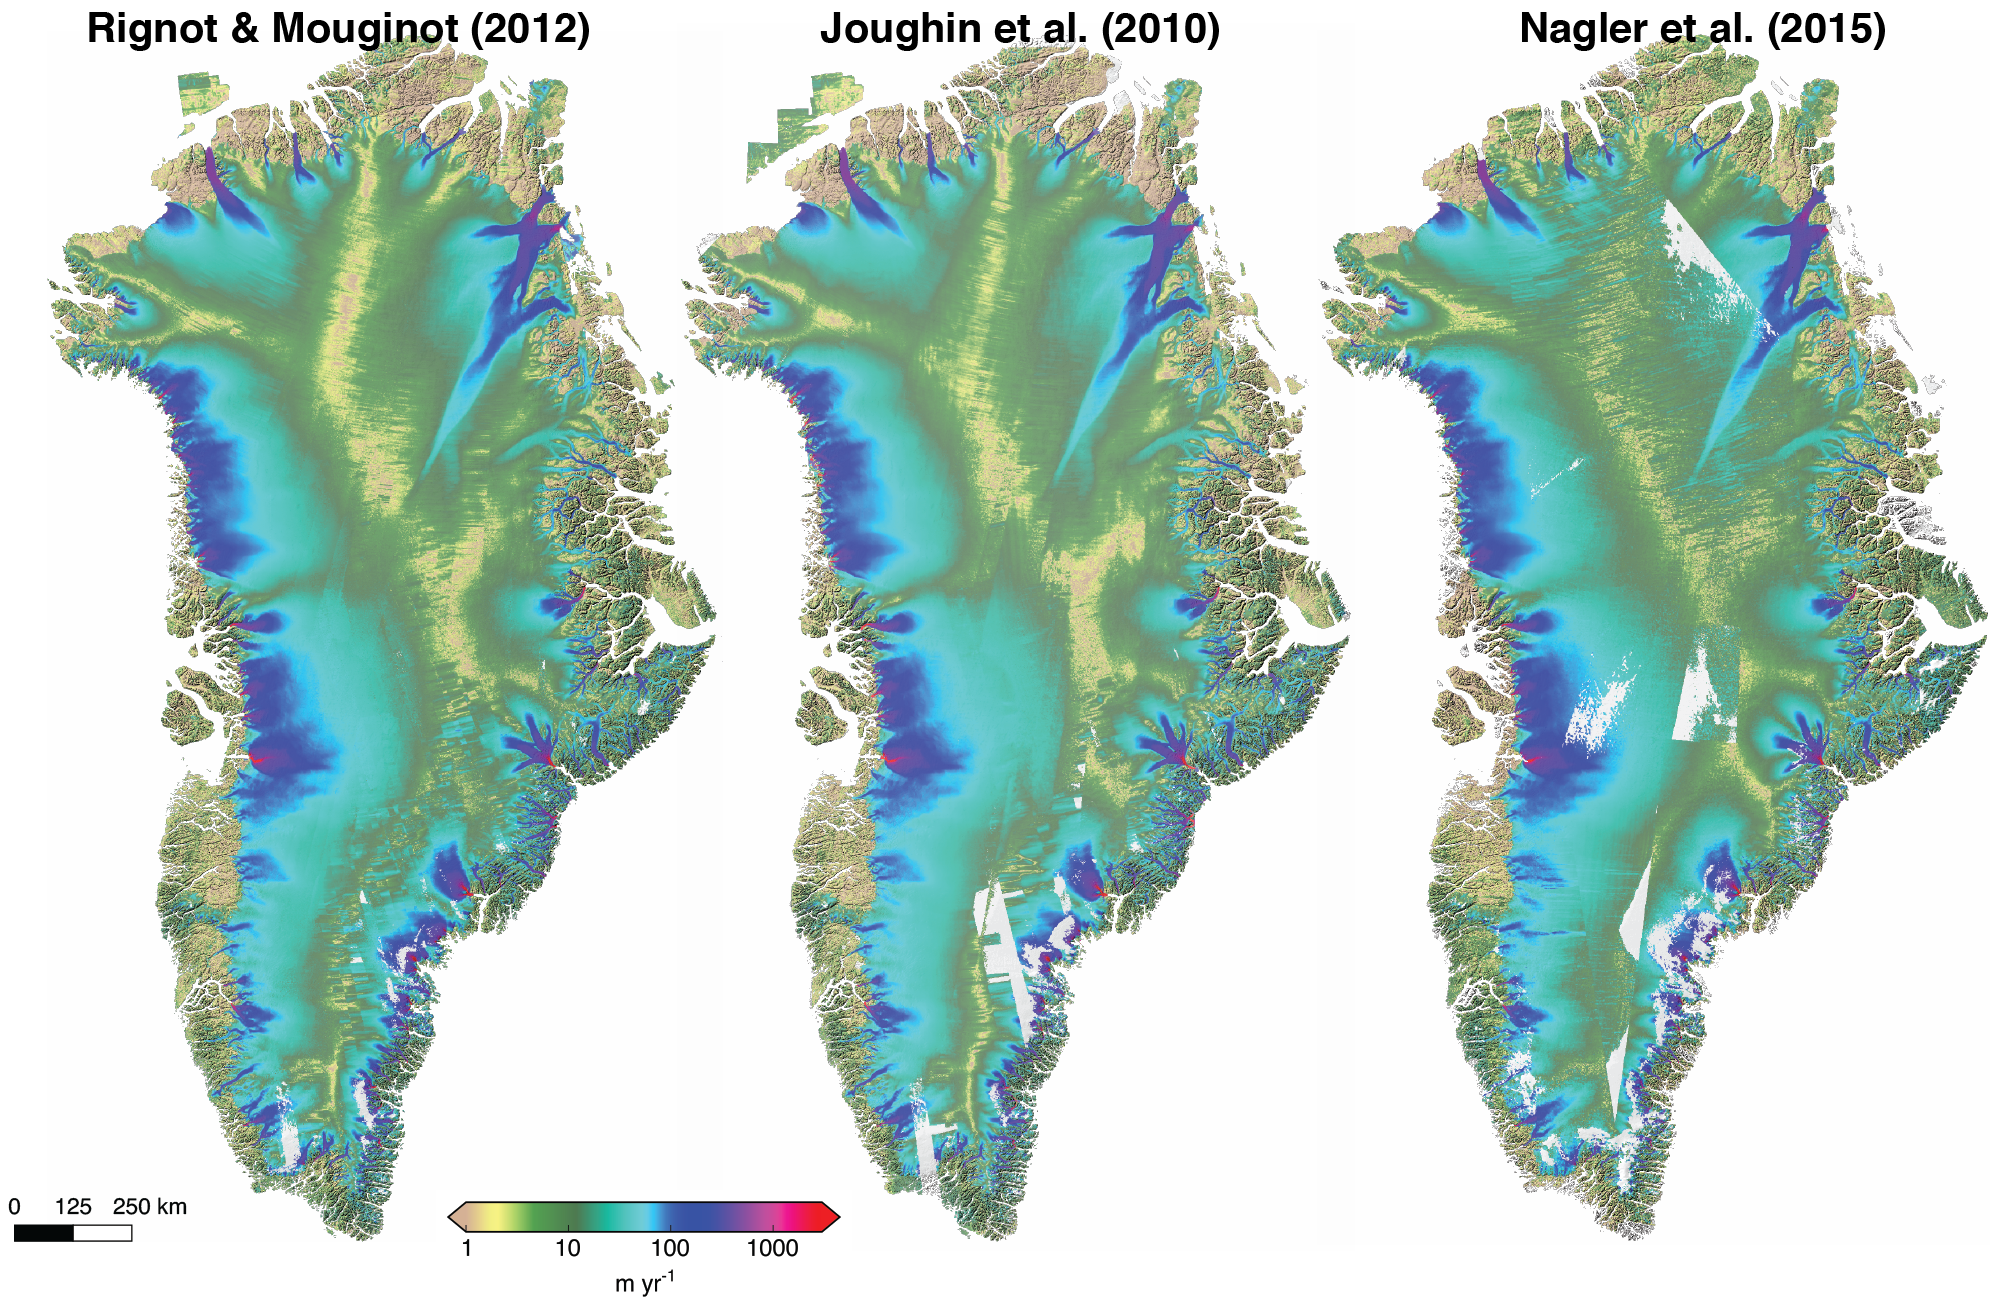
\includegraphics[height=.7\textheight]{greenland-sar-3}
 \end{figure}
\end{frame}

\begin{frame}{Observed temporal flow variability}
  increasing temporal variability using TerraSar-X/Tandem-X, Sentinel but also from optical imagery (worldview, Landsat8)
  \begin{figure}
    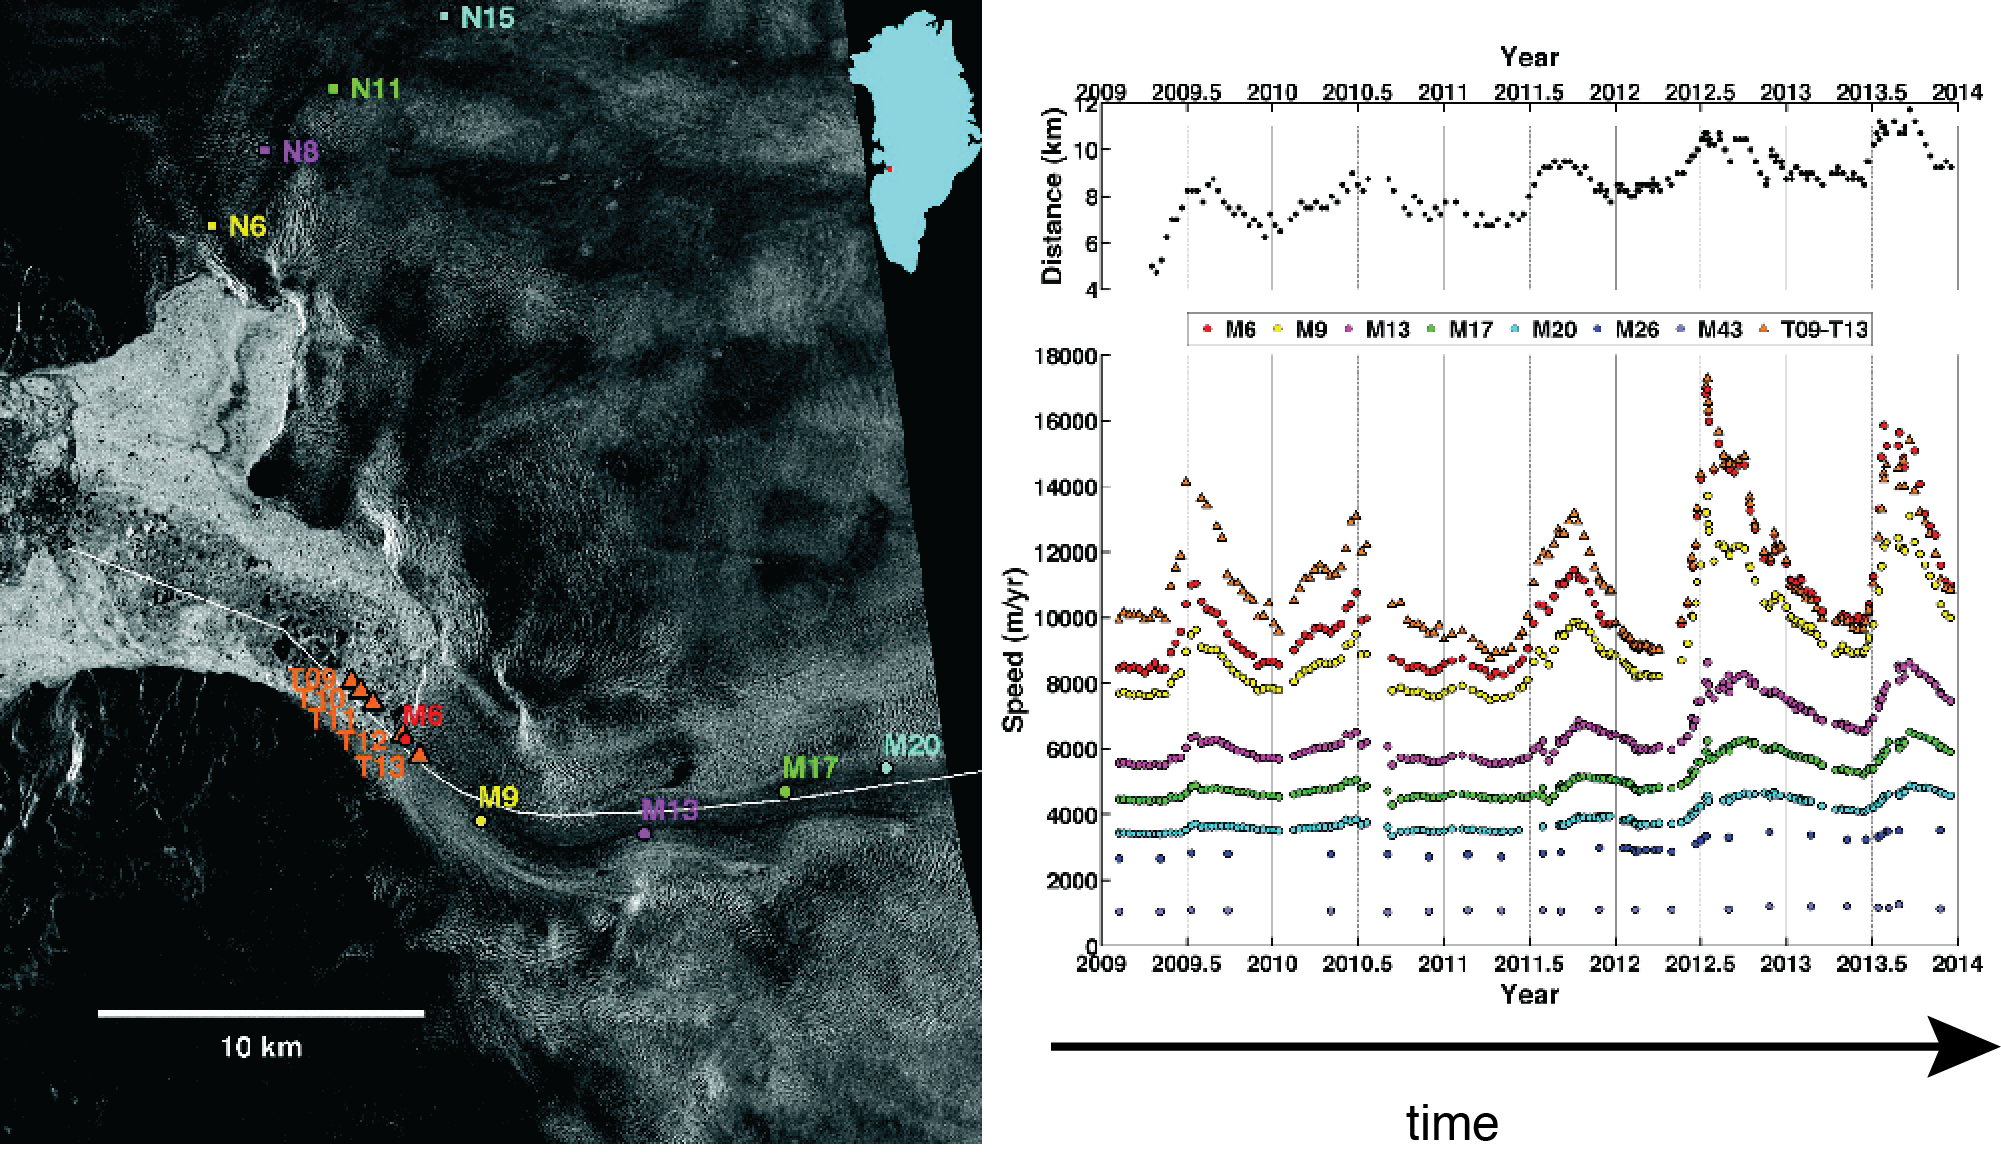
\includegraphics[height=.7\textheight]{joughin-2014-collage}
 \end{figure}
\end{frame}


\setbeamertemplate{background canvas}
  {
     \tikz{\node[inner sep=0pt,opacity=.3] {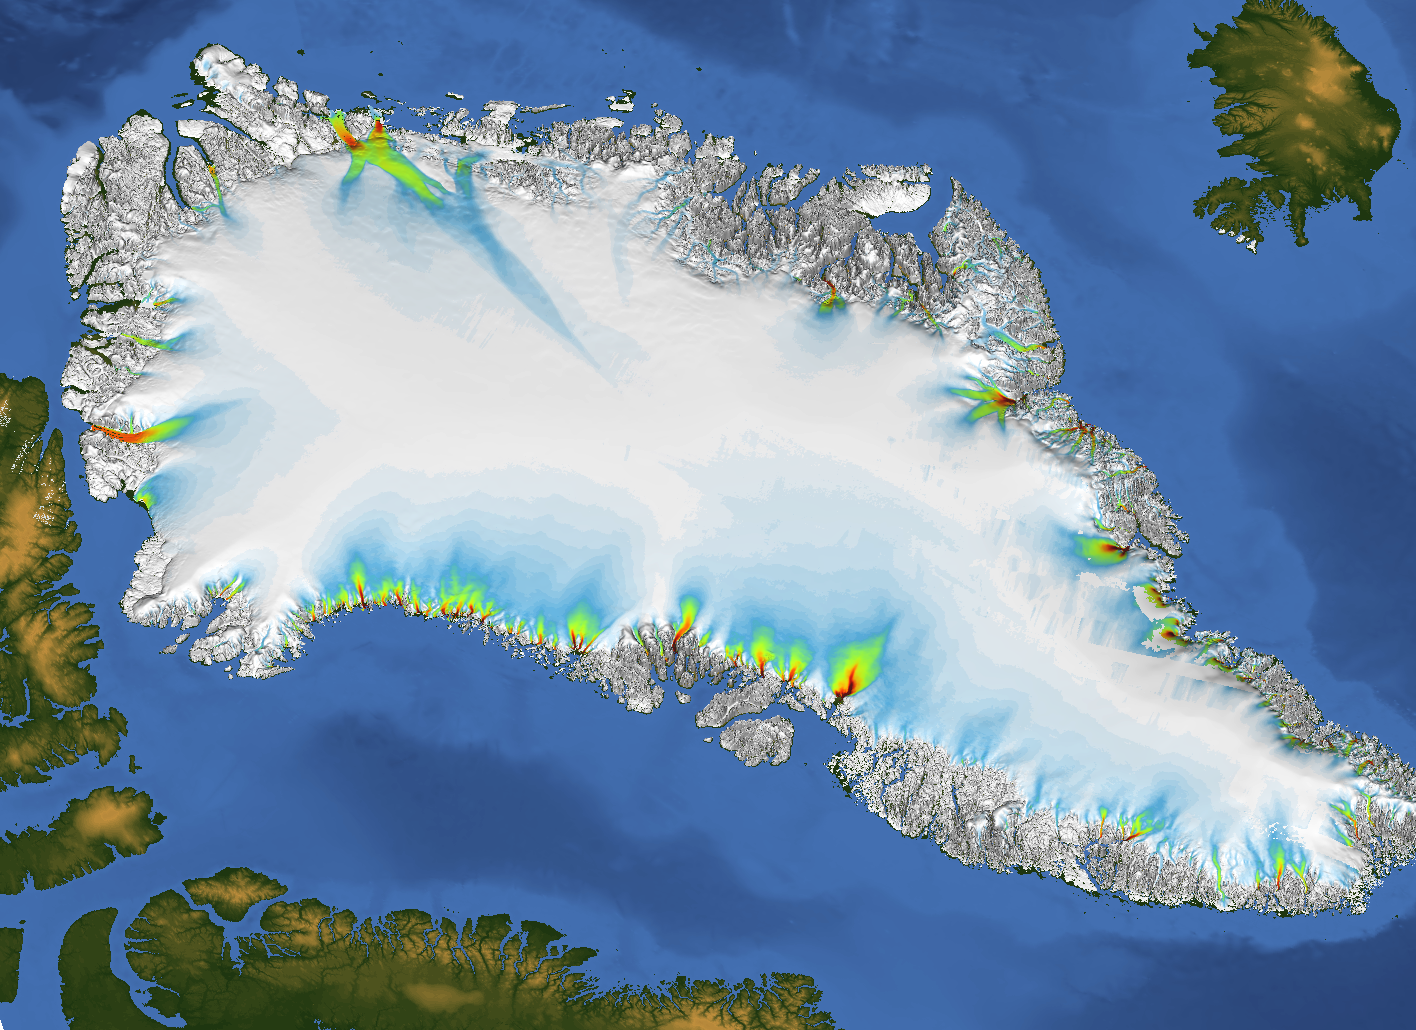
\includegraphics[height=\paperheight,width=\paperwidth]{grn_iss}};}
} 


\begin{frame}[plain]
  \begin{transbox}[0.8]
    \begin{block}{We note}
      \begin{itemize}
      \item any credible modeling effort must be able to explain this variability
      \item ice thickness is a leading order constraint on flow
      \end{itemize}
    \end{block}
  \end{transbox}
\end{frame}


\setbeamertemplate{background canvas}
{
%
} 

\begin{frame}{Flow speeds}
\vspace{-0.74em}
  \begin{columns}
    \column[c]{5cm}
    \begin{figure}
      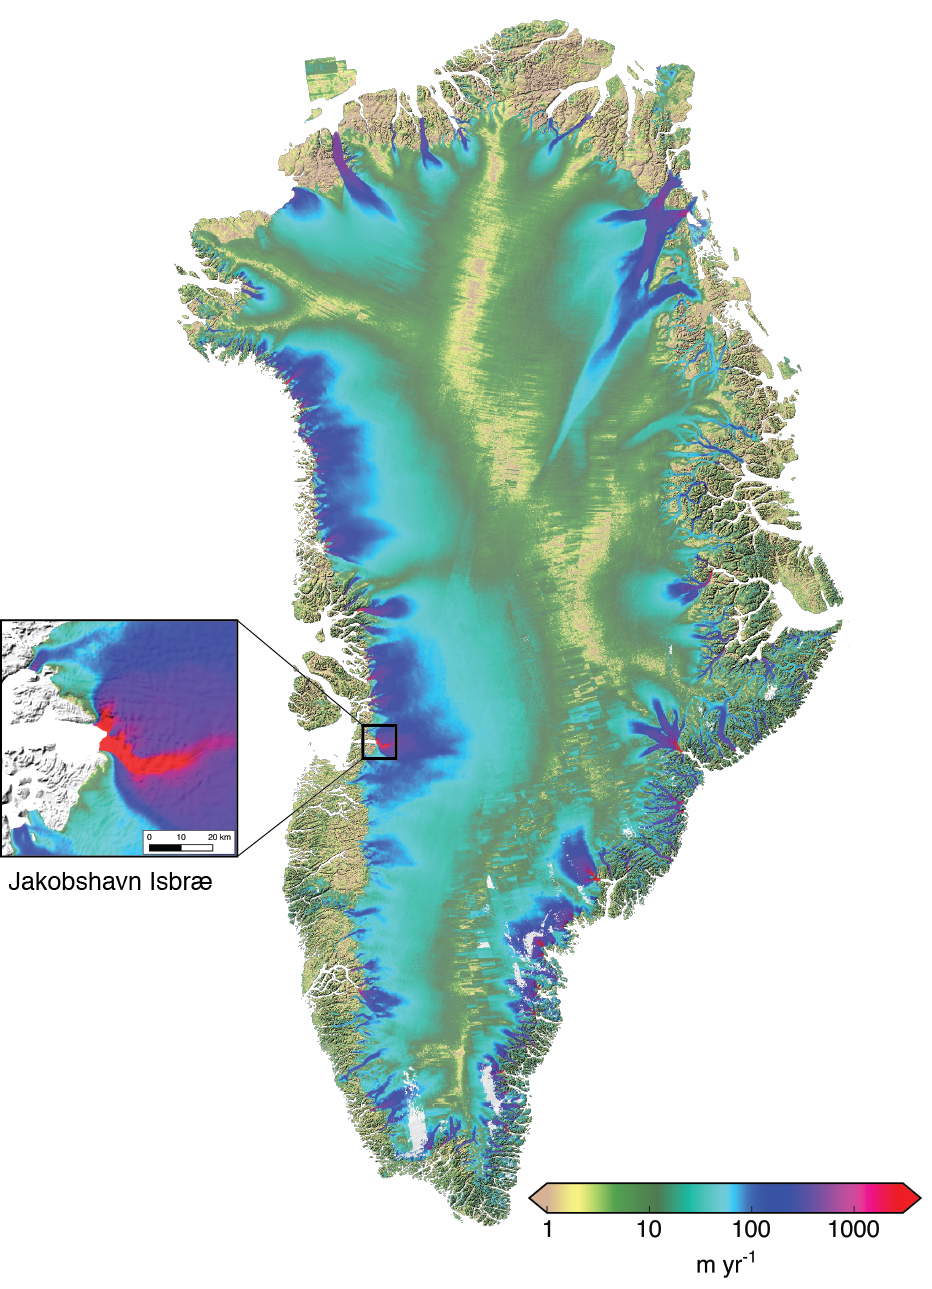
\includegraphics[width=\textwidth]{greenland-obs-overview}
    \end{figure}
    \column[c]{5cm}
    \only<1>{Jakobshavn Isbr{\ae}}
    \includegraphics<1>[width=\textwidth]{jakobshavn-obs-nogate}
    \only<1>{\\ {} }
  \end{columns}
\end{frame}


\begin{frame}{Ice thickness map until 2013/14}
\vspace{-0.74em}
  \begin{columns}
    \column[c]{5cm}
    \begin{figure}
      \includegraphics[width=\textwidth]{greenland-obs-basal-overview}
    \end{figure}
    \column[c]{5cm}
    \only<1>{Jakobshavn Isbr{\ae}}
    \only<2>{no fast flow}
    \includegraphics<1>[width=\textwidth]{jakobshavn-bed-5000m-ba01}
    \includegraphics<2>[width=\textwidth]{jakobshavn-speed-exp-4500m-ba01}
    \only<1>{\\ 5\,km, Bamber et al. (2001)}
    \only<2>{\\ simulated surface speed}
  \end{columns}
\end{frame}


\begin{frame}
\begin{block}{Pre-2016 Conclusion}
  \begin{itemize}
  \item outlet glacier flow cannot be reproduced using coarse resolution SIA models and by tuning just a few scalar ice-sheet wide tuning parameters
  \end{itemize}
\end{block}
\begin{block}{Consequence}
  \begin{itemize}
  \item IPCC AR4 excluded sea-level rise projections for ice sheet models because \alert{``\ldots but recent changes in ice sheet margins and ice streams cannot be simulated accurately with these models, demonstrating a need for resolving the full stress configuration.''}
  \end{itemize}
\end{block}
\begin{block}{Suggested remedy}
  \begin{itemize}
  \item develop models that solve the Stokes momentum balance or at least a higher-order approximation thereof
  \item use surface observations (flow velocities) to invert for the unknown basal traction
  \end{itemize}
\end{block}
\end{frame}


\begin{frame}{Post-AR4 model development frenzy}
  \begin{itemize}
    \item in the wake of AR4, new FEM-based open-source higher-order and Stokes model emerge featuring advanced data assimilation capabilities such as ELMER, ISSM, VarGlas
  \end{itemize}
  \shadowimage[width=\textwidth]{fem-models}
\end{frame}


\begin{frame}{Post-AR4 model development frenzy}
  \vspace{-0.74em}
  \begin{columns}
    \column[c]{5.25cm}
    \begin{figure}
      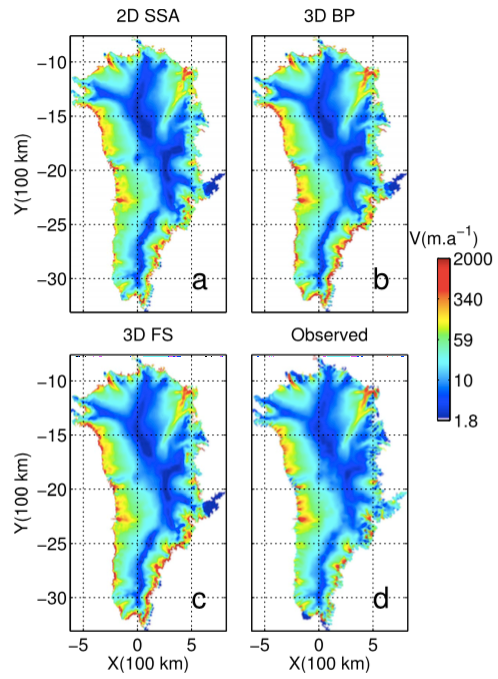
\includegraphics[width=\textwidth]{larour-2012-fig8}
      \caption{ISSM, Larour et al. (2012), Fig.~8}
    \end{figure}
    \column[c]{7cm}
  \begin{itemize}
  \item by construction, using inversion of surface velocities results in good agreement between observed and simulation surface velocities
  \end{itemize}
  \end{columns}
\end{frame}


\begin{frame}{Where we are}
  \begin{itemize}[<+-| alert@+>]
  \item using sparse observations of ice thickness, outlet glacier flow cannot be reproduced \emph{WITHOUT} inversion of surface velocities (i.e. tuning a very large number of basal parameters)
  \item I'm not going to talk why inversion is less desirable than using just a few scalar ice-sheet wide tuning parameters except:
  \item \bf{With four parameters I can fit an elephant, and with five I can make him wiggle his trunk.} (John von Neumann)
  \item higher-order and Stokes models remain computationally too expensive for century-scale simulations at high grid resolutions
  \end{itemize}
  \begin{figure}
    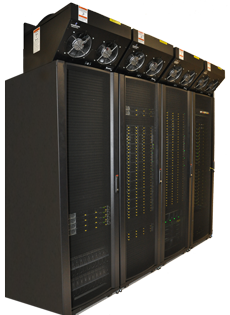
\includegraphics[height=2.5cm]{pacman} \qquad
    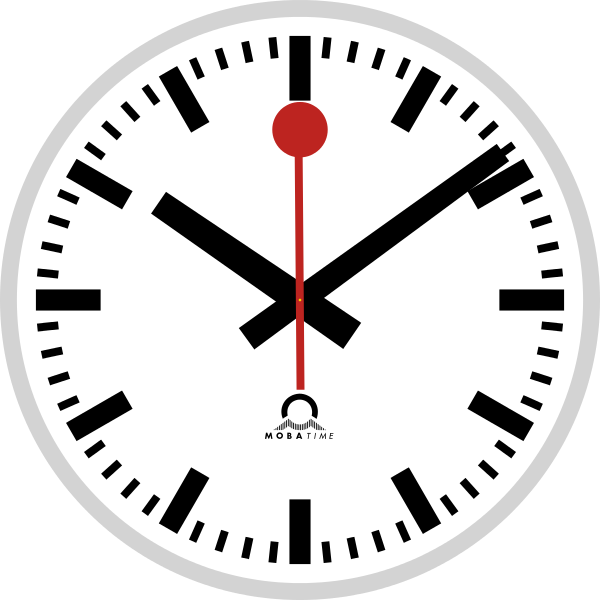
\includegraphics[height=2.5cm]{swiss_railway_clock} \qquad
    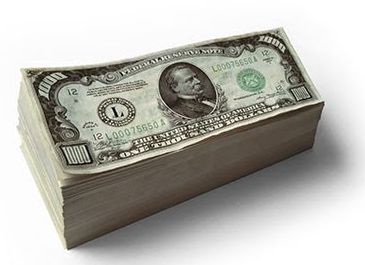
\includegraphics[height=2.5cm]{1000-dollar-bills}
  \end{figure}
\end{frame}


\begin{frame}{Where we need to go}
  \begin{block}{We explain the complex flow patterns using accurate, dense ice thickness measurements}
    \begin{itemize}
    \item with a computationally-efficient high-resolution ice sheet model
    \item coupled to uniformly applied models of subglacial hydrology and basal sliding?
    \end{itemize}
  \end{block}
\end{frame}


\begin{frame}{NASA Operation IceBridge}
  \vspace{-0.74em}
  \begin{columns}
    \column[c]{2cm}
    
\includegraphics[width=\textwidth]{nasa-logo} \\
    
\includegraphics[width=\textwidth]{oib}
    \column[c]{10cm}
    \begin{itemize}
    \item NASA realized that collecting a lot more ice thickness measurements is crucial to make ice sheet models better
    \item ice thickness measurements using the CReSIS radar became an important part of their Operation IceBridge mission (2009--today)
    \end{itemize}
  \end{columns}
\end{frame}


\begin{frame}{NASA Operation IceBridge}
\vspace{-0.74em}
  \begin{columns}
    \column[c]{2.5cm}
    \only<1>{2001}
    \only<2>{from 2009 on}
    \only<3>{2014}
    \column[c]{6cm}
    \begin{figure}
      \includegraphics<1>[height=8cm]{greenland-bed-old}
      \includegraphics<2>[height=8cm]{greenland-bed-old-oib}
      \includegraphics<3>[height=8cm]{greenland-bed-mcb}
    \end{figure}
  \end{columns}
\end{frame}

\begin{frame}{Zoom in to Jakobshavn Isbr{\ae}}
  \begin{figure}
    \small{Bamber (2001) \hspace{5em} Morlighem (2014)}
    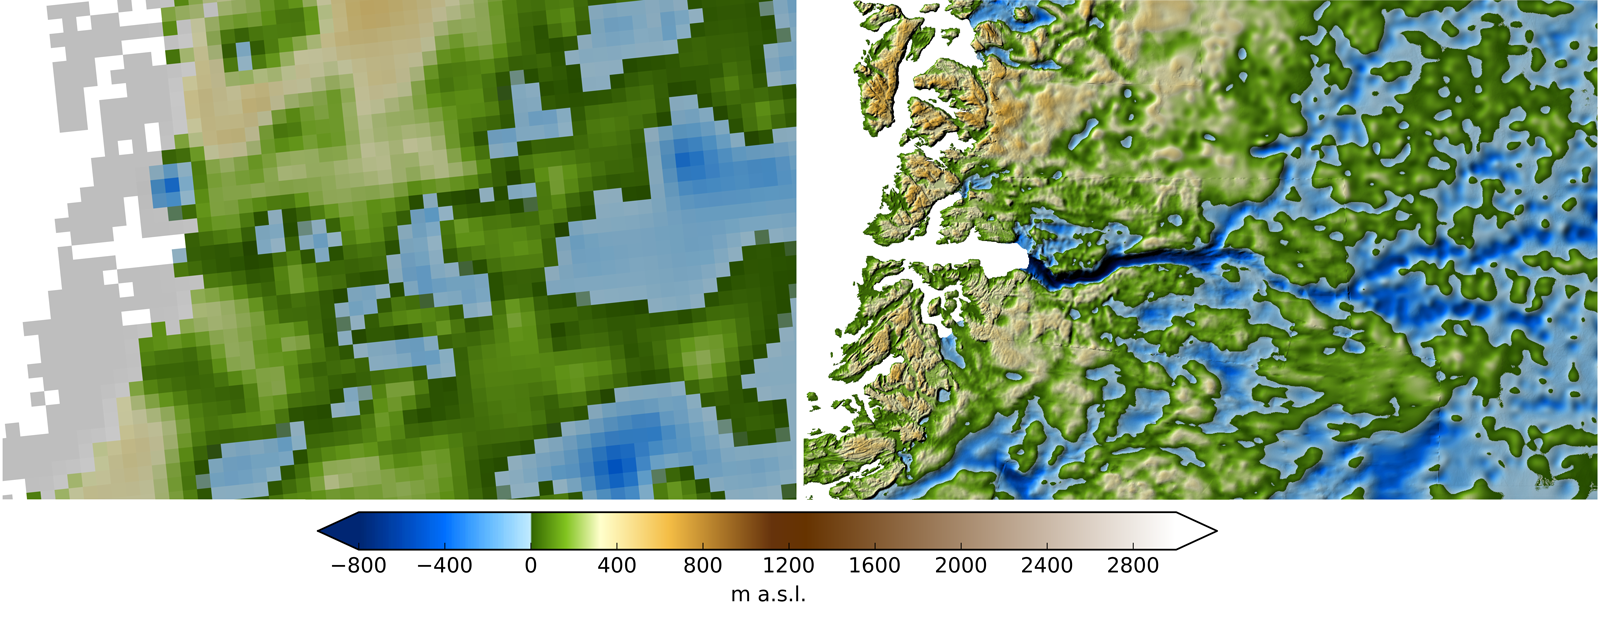
\includegraphics[width=12cm]{jako_bed}
 \end{figure}
\end{frame}


\begin{frame}{NASA Operation IceBridge}
  \begin{columns}
    \column[c]{8cm}
    \begin{figure}
      \small{Bamber (2001) \hspace{4em} Morlighem (2014)}
      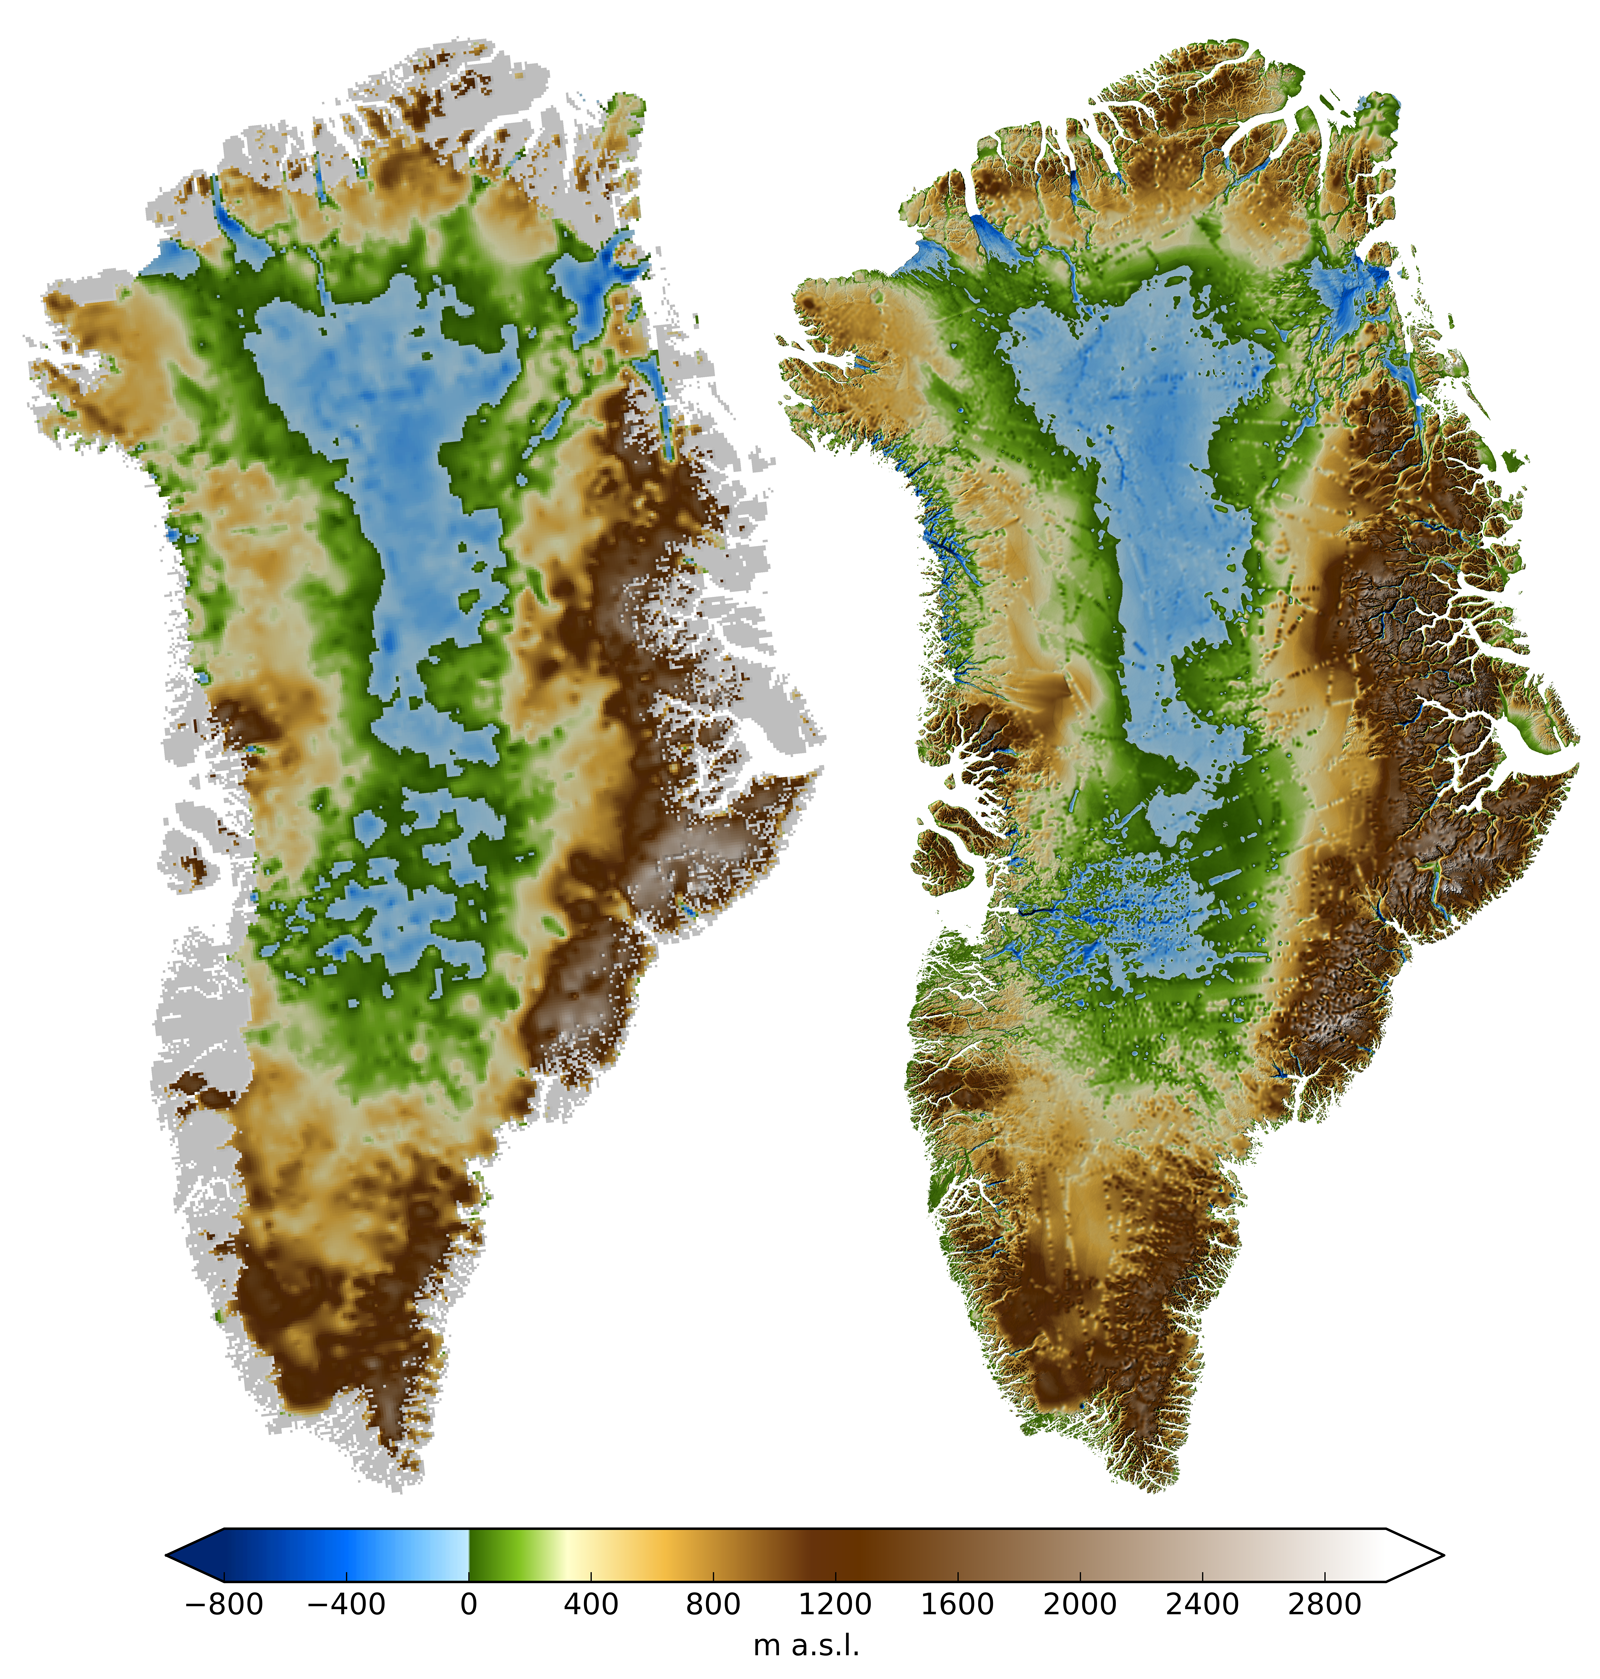
\includegraphics[height=7.5cm]{greenland_bed}
    \end{figure}
    \column[c]{4cm}
    \begin{itemize}
    \item from 5\,km to 150\,m horizontal grid resolution
    \end{itemize}
  \end{columns}
\end{frame}

\begin{frame}{NASA Operation IceBridge}
  \begin{figure}
    
\includegraphics[height=2.5cm]{nasa-logo} \qquad
    
\includegraphics[height=2.5cm]{oib} \qquad
    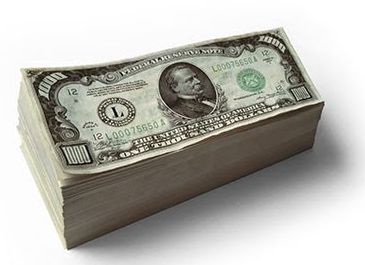
\includegraphics[height=2.5cm]{1000-dollar-bills}
  \end{figure}
  \begin{itemize}
  \item do NASA's OIB million\$ really make ice sheet models better?
  \item use your favorite high resolution ice sheet model to find out
\end{itemize}
\end{frame}


\begin{frame}{Validation metrics: flow through flux gates}
  \vspace{-1em}
  \begin{columns}
    \column[c]{4cm}
    \begin{figure}
      \includegraphics<1>[width=3cm]{upernavik-gate-zoom}
    \end{figure}
    \begin{figure}
      \includegraphics<1>[width=4cm]{Kong_Oscar_Gletscher_velsurf_normal_profile_250m_greenland_2008-2009_grid_mo14_flow_sel_green}
    \end{figure}
    \column[c]{7cm}
    \begin{figure}
      \includegraphics<1>[height=7.5cm]{greenland-gates-29}
    \end{figure}
  \end{columns}
\end{frame}


\begin{frame}{Validation metrics: flow through flux gates}
  \vspace{-1em}
  \begin{columns}
    \column[c]{4cm}
    \begin{figure}
      \includegraphics<1>[width=3cm]{upernavik-gate-zoom}
    \end{figure}
    \begin{figure}
      \includegraphics<1>[width=4cm]{Kong_Oscar_Gletscher_velsurf_normal_profile_250m_greenland_2008-2009_grid_mo14_flow_sel_green}
    \end{figure}
    \column[c]{7cm}
    \begin{block}{Metrics of success}
      \begin{itemize}
      \item assess model performance by comparing observed and simulated surface velocities along cross-flow profiles of 29  outlet glaciers
      \item quantify model's ability to capture the spatial variation in flow structure using \vspace{-.75em}
        \begin{itemize}
        \item the Pearson $r$ correlation coefficient and 
        \item the r.m.s. difference
        \end{itemize}
        between observations and simulations along the 29 profiles
      \item evaluate every 250\,m \alert{$\Rightarrow$ gates as shapefiles available on github}
      \end{itemize}
    \end{block}
  \end{columns}
\end{frame}


\begin{frame}{Model setup}
  
\includegraphics[width=4cm]{pism-logo}
  \begin{itemize}
  \item this study is not about PISM
  \item any ISM capable of <1\,km grid resolution will do
  \item enthalpy field from a paleo-climate initialization
  \item calculate diagnostic velocity fields that correspond to a given geometry using flux correction method
  \end{itemize}
\end{frame}


\begin{frame}{Model calibration at 1,500\,m resolution}
  \vspace{-.5em}
  \begin{columns}
    \column[c]{6.5cm}
    \begin{figure}
      \includegraphics[width=\textwidth]{calib-speeds}
    \end{figure}
    \column[c]{5.5cm}
    \begin{itemize}
    \item 15 simulations to explore parameter space (sliding law exponent $q$, enhancement factor $E$, SSA flow law exponent $n$)
    \item choose simulation with smallest r.m.s. difference
    \end{itemize}
  \end{columns}
\end{frame}

\begin{frame}{Model calibration at 1,500\,m resolution}
  \vspace{-.5em}
  \begin{columns}
    \column[c]{5cm}
    \begin{figure}
      \includegraphics<1>[width=\textwidth]{calib-speed-010-3}
      \includegraphics<2>[width=\textwidth]{calib-speed-025-3}
      \includegraphics<3>[width=\textwidth]{calib-speed-033-3}
      \includegraphics<4>[width=\textwidth]{calib-speed-050-3}
      \includegraphics<5>[width=\textwidth]{calib-speed-060-325}
      \includegraphics<6>[width=\textwidth]{calib-speed-080-3}
    \end{figure}
    \column[c]{5.5cm}
    \begin{itemize}
    \item general flow pattern well reproduced by all simulations
    \item slow flow in the interior, fast flow in outlet glaciers
    \item results more sensitive to ice thickness than to ice dynamics
    \item<6> results are very robust
    \end{itemize}
  \end{columns}
\end{frame}


\begin{frame}{Best simulation}
  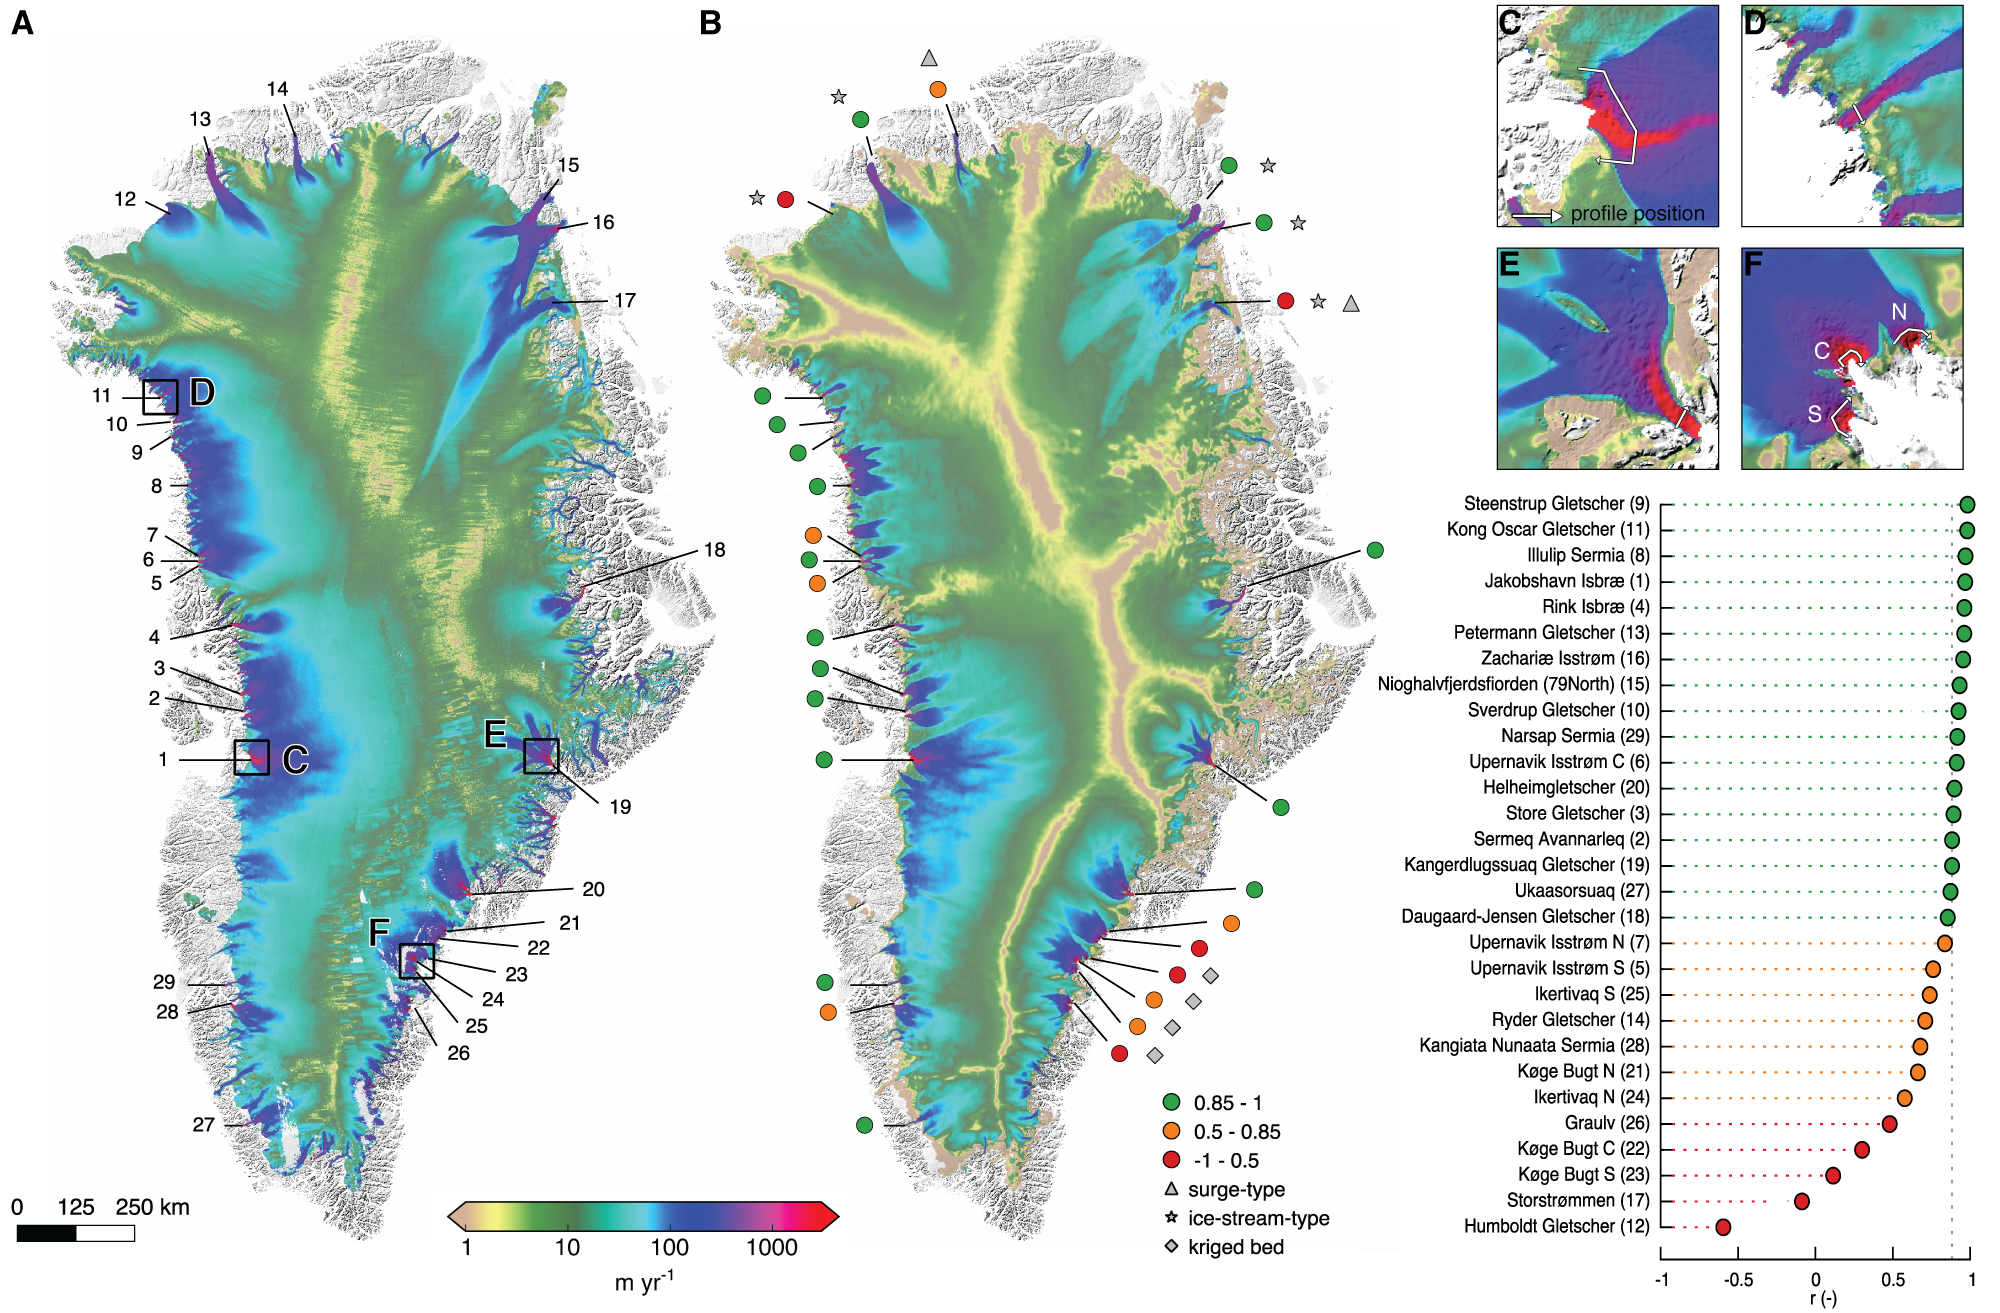
\includegraphics[height=8cm]{greenland-overview-3}
\end{frame}

\begin{frame}{Role of model resolution}
  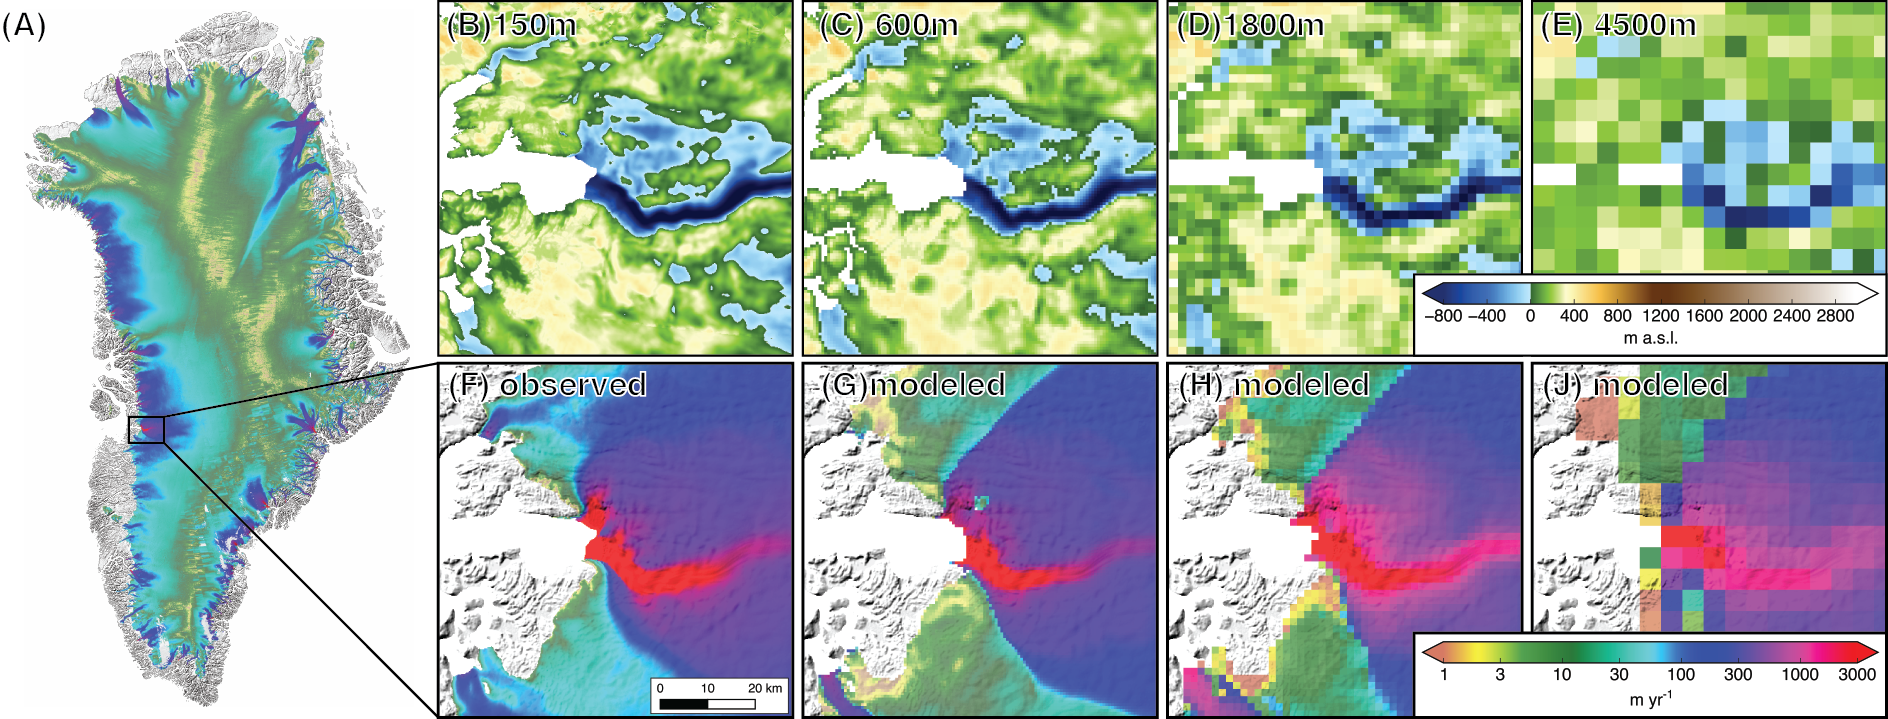
\includegraphics[width=\textwidth]{jakobshavn-beds}
\end{frame}

\begin{frame}{Role of model resolution}
  \begin{figure}
    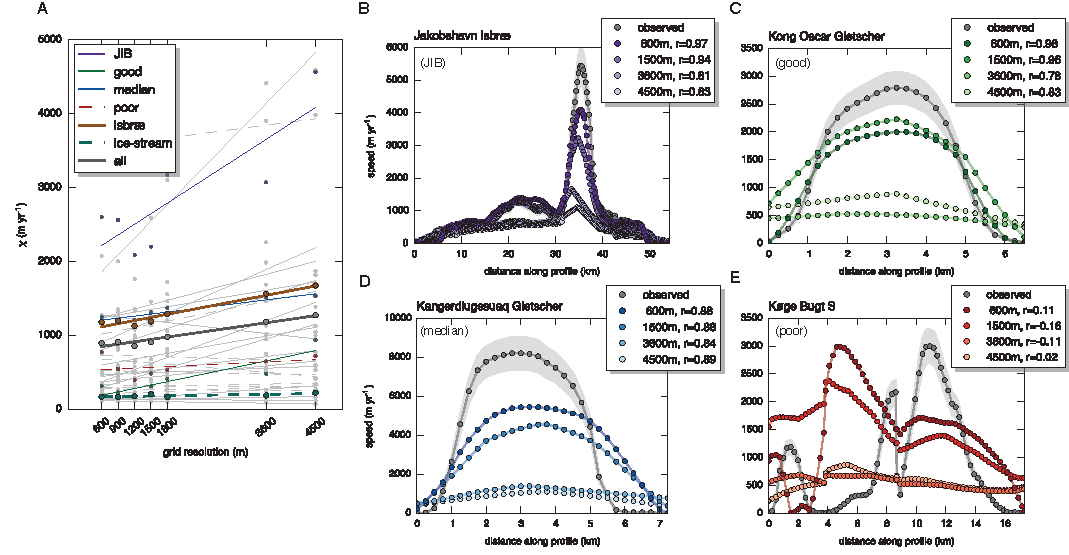
\includegraphics[height=6cm]{grid-resolution-4}
  \end{figure}
\end{frame}


\begin{frame}{Role of ice thickness}
  \begin{figure}
    \includegraphics<1>[width=\textwidth]{nw-coast-1-4500m-ba2001-01}
    \includegraphics<2>[width=\textwidth]{nw-coast-1-4500m-mo2014-01}
    \includegraphics<3>[width=\textwidth]{nw-coast-1-600m-ba2001-01}
    \includegraphics<4>[width=\textwidth]{nw-coast-1-600m-mo2014-01}
    \\[1em]
    \only<1>{low model and low data set resolution}
    \only<2>{low model and high  data set resolution}
    \only<3>{high model and low data set resolution}
    \only<4>{high model and high data set resolution}
  \end{figure}
\end{frame}

\begin{frame}{Role of ice thickness}
  \begin{figure}
    \includegraphics<1>[width=\textwidth]{nw-coast-1-600m-mo2014-01}
  \end{figure}
      \begin{itemize}
        \item only {\bf high} \alert{model} and \alert{data} set resolution result in outlet glacier flow
      \end{itemize}
\end{frame}


\setbeamertemplate{background canvas}
  {
     \tikz{\node[inner sep=0pt,opacity=.5] {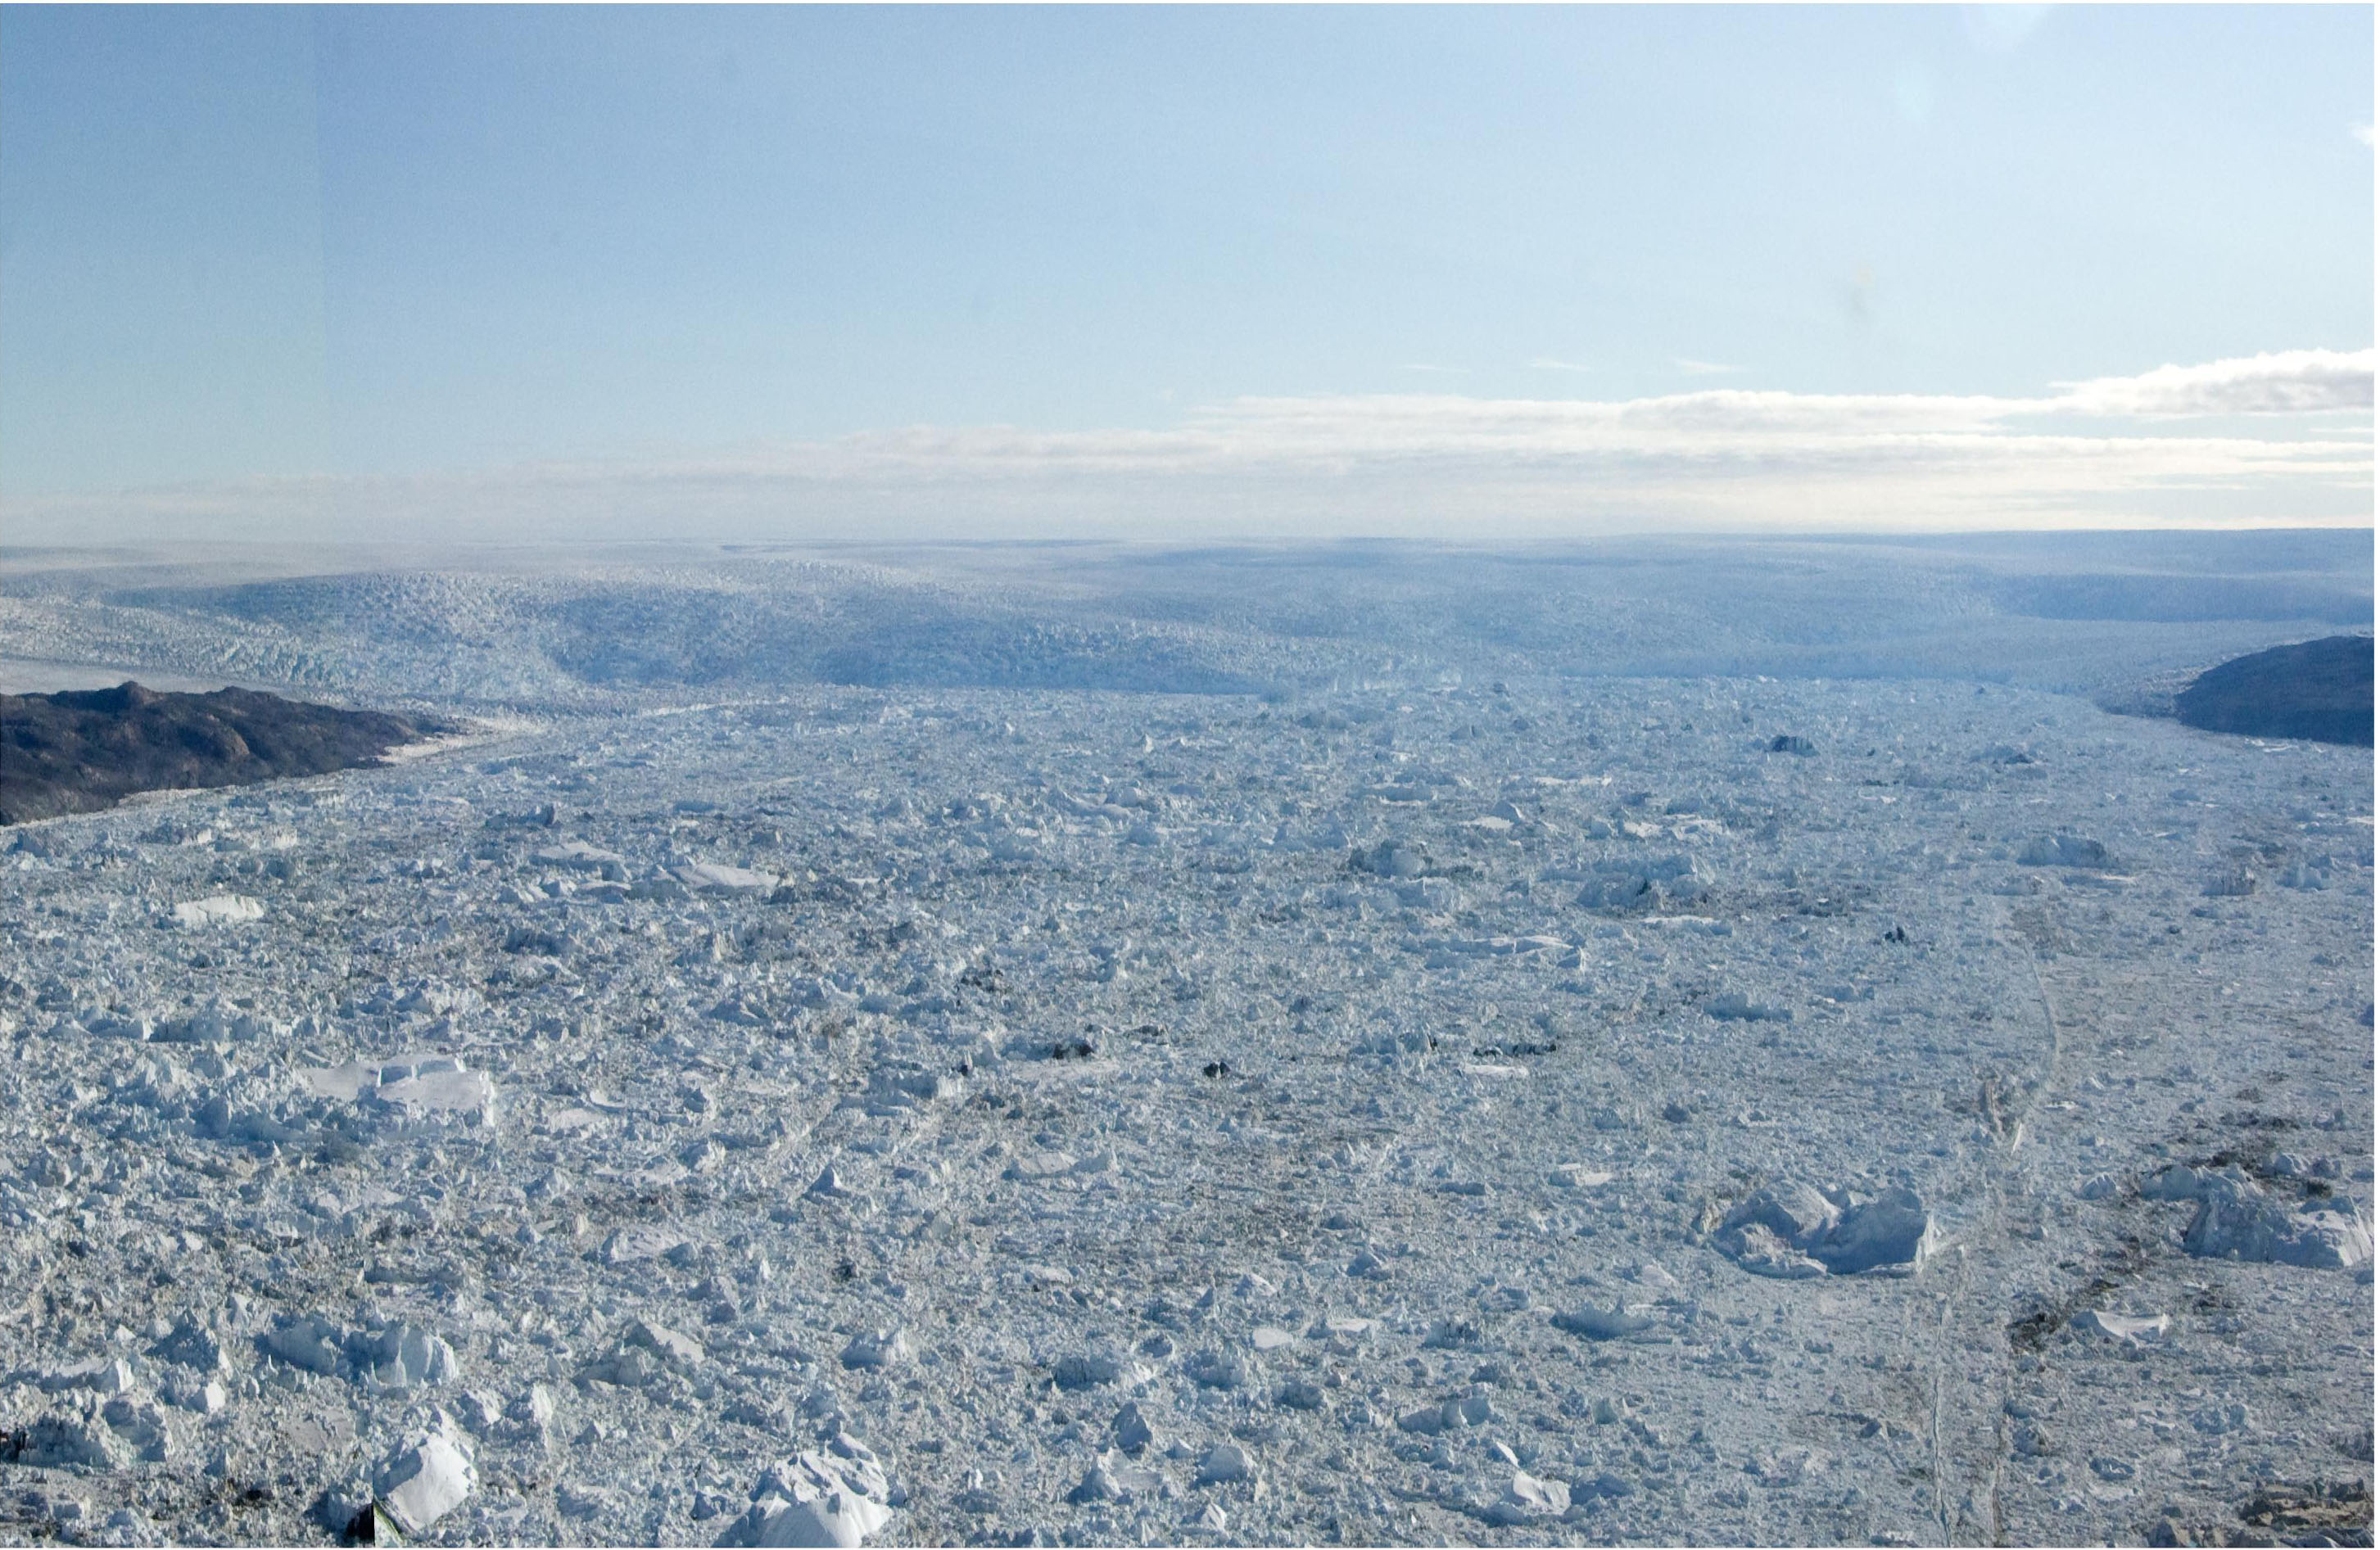
\includegraphics[height=\paperheight,width=\paperwidth]{jakobshavn-2007}};}
} 

\begin{frame}[plain]
  \begin{transbox}[0.8]
  \begin{block}{Ice stream-type glaciers}
    glaciers are characterized by low-surface slopes and low driving stresses (Antarctic ice streams, Humboldt Gletscher, NEGIS)
  \end{block}
  \begin{block}{Isbr{\ae}-type glaciers}
    glaciers flow through channels significantly deeper than the surrounding ice (the remainder of GrIS's outlet glaciers)
  \end{block}
  \vspace{1em}
  after Truffer \& Echelmeyer (2003)
  \end{transbox}
\end{frame}

\setbeamertemplate{background canvas}
{
%
} 


\begin{frame}{Role of flow type}
  \begin{columns}
    \column[c]{5.5cm}
    \begin{figure}
      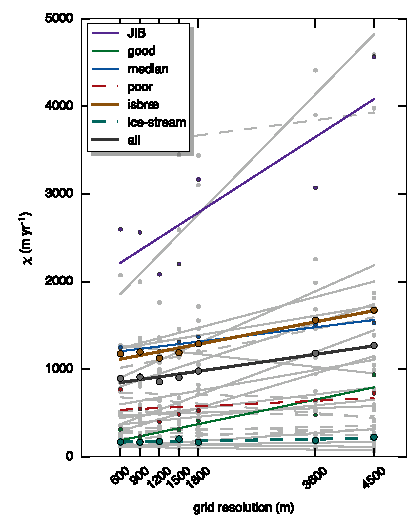
\includegraphics[width=5.5cm]{rmsd_regression_velsurf_normal_250m_grid_mo14_flow_combined}
    \end{figure}
    \column[c]{6.5cm}
    \begin{itemize}
      \item not all isbr{\ae}-type glaciers benefit from grid refinement
      \item ice stream-type glaciers do not benefit from grid refinement
    \end{itemize}
  \end{columns}
\end{frame}


\begin{frame}{Role of flow type: isbr{\ae}-type glaciers}
    \begin{figure}
      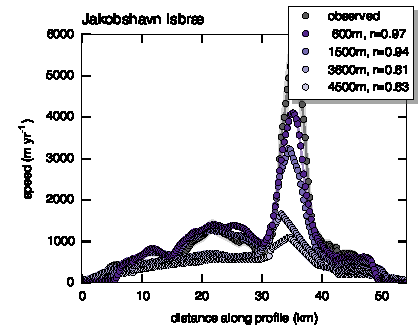
\includegraphics[width=7cm]{Jakobshavn_Isbrae_velsurf_normal_profile_250m_greenland_2008-2009_grid_mo14_flow_sel_purple}
    \end{figure}
    \begin{itemize}
      \item most isbr{\ae}-type glaciers benefit from grid refinement
    \end{itemize}
\end{frame}


\begin{frame}{Role of flow type: ice stream-type glaciers}
  \begin{columns}
    \column[c]{5.5cm}
    \begin{figure}
      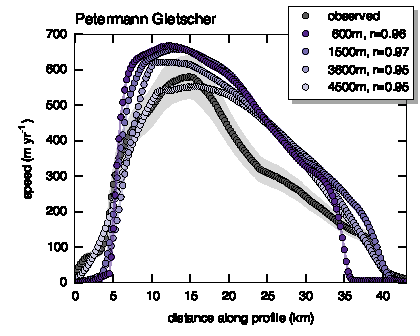
\includegraphics[width=5.5cm]{Petermann_Gletscher_velsurf_normal_profile_250m_greenland_2008-2009_grid_mo14_flow_sel_purple}
    \end{figure}
    \column[c]{6.5cm}
    \begin{itemize}
      \item ice stream-type glaciers do not benefit from grid refinement
    \end{itemize}
  \end{columns}
\end{frame}


% \begin{frame}{Glaciers with few ice thickness measurements}
%   \begin{columns}
%     \column[c]{5.5cm}
%     \begin{figure}
%       \includegraphics[width=5.5cm]{Koge_Bugt_C_velsurf_normal_profile_250m_greenland_2008-2009_grid_mo14_flow_sel_purple}
%     \end{figure}
%     \column[c]{6.5cm}
%     \begin{itemize}
%       \item these glaciers are poorly captured at all grid resolutions
%       \item more measurements are needed
%     \item in general glaciers with dense observations are modeled well (e.g. Jakobshavn Isbr{\ae} while glaciers with limited coverage are modeled poorly (e.g. K{\o}ge Bugt)
%     \end{itemize}
%   \end{columns}
% \end{frame}


\begin{frame}{What really matters  \ldots using Ed's words}
  \begin{enumerate}
    \item an accurate map of subglacial topography
    \item a stress regime in which viscous membrane stresses are part of the balance with basal sliding resistance
    \item an energy-conservation-driven basal stress model derived (conceptually) from a model of a wet, pressurized, deformable basal layer
    \item  high model resolution over all areas of the ice sheet where sliding is possible and/or steep/rough basal topography exists
  \end{enumerate}
\end{frame}


\begin{frame}{Conclusions}
  \begin{itemize}
    \item first time that the general flow patterns are captured for the {\bf right} reason
    \item for isbr{\ae}-type glaciers ice thickness matters the most, subglacial hydrology comes later
    \item this is very encouraging
    \item opens the door for prognostic simulations using simple models of subglacial hydrology
  \end{itemize}
\end{frame}


\begin{frame}{Final Remarks}
  \begin{itemize}
    \item we don't get Humboldt Gletscher and NEGIS right. \alert{Fahnestock hypothesis:} related to (thermal) history
    \item some of the remaining discrepancies could also be attributed to limited knowledge of ice thickness in the vast interior of Greenland
    \item we get good results using a shallow model that includes vertical shearing and horizontal membrane stresses
    \item IPCC AR4's \alert{``\ldots but recent changes in ice sheet margins and ice streams cannot be simulated accurately with these models, demonstrating a need for resolving the full stress configuration.''} was formulated in a somewhat unfortunate way
  \end{itemize}
\end{frame}

\begin{frame}{Final Remarks}
  \begin{itemize}
    \item ice thickness mapping by NASA's OIB and similar efforts are paying off big time
    \item similar efforts are suggested for Antarctica
  \end{itemize}
\end{frame}


\begin{frame}{Final Remarks}
\begin{columns}
  \column[c]{3cm}
  \begin{figure}
    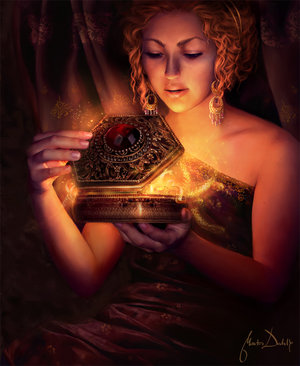
\includegraphics[width=1.75cm]{pandoras-box}
  \end{figure}
  \column[c]{8cm}
  The days of coarse ($>$1\,km) resolution Greenland models are over
\end{columns}
\end{frame}



% \begin{frame}{Conclusions}
% We now can
% \begin{itemize}
% \item \alert{measure} improvements that both better observations and better models bring
% \item \alert{determine} the grid resolution needed to model a particular outlet glacier accurately
% \item flux \alert{profiles} are a better metric than the total flux
% \end{itemize}
% \begin{columns}
%   \column[c]{3cm}
%   \begin{figure}
%     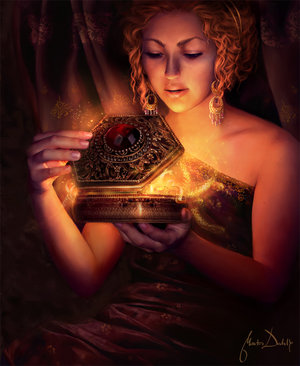
\includegraphics[width=1.75cm]{pandoras-box}
%   \end{figure}
%   \column[c]{8cm}
%   There is no going back to coarse resolution
% \end{columns}
% \begin{block}{Ice Sheet Model?}
% \begin{itemize}
% \item this is a general validation method independent of the underlying ice sheet model
% \end{itemize}
% \end{block}
% \end{frame}


\end{document}
